\chapter{Background} \label{ch:background}

This section provides the key background knowledge that motivates the design choices and the biology behind the models developed. Whilst self-evident, the biology and theory are increasingly complex the more we explore them, and it should be noted that the mechanisms discussed are often simplified

\section{Auditory Cues and Echolocation}

Much like sonar, bats send out sound waves to reflect off of prey in an active acoustic sensing strategy called echolocation (i.e. locating with echoes). This is different from the passive sound localisation that most other mammals do, which entirely depends on external ambient sounds. The active nature of echolocation means the bat can have control and knowledge of the signal it is sending out, and so can observe changes to this signal in order to infer the location of objects, such as insects. These changes, or auditory cues, are essentially the features extracted from the returned echo for the bat's brain to infer the location, much like a typical signal processing problem. We can group these auditory cues for their use in estimating our three coordinates of distance, azimuth, and elevation. These establish the baseline signal processing problems that biological neural architectures must solve.

\begin{figure}[H]
    \centering
    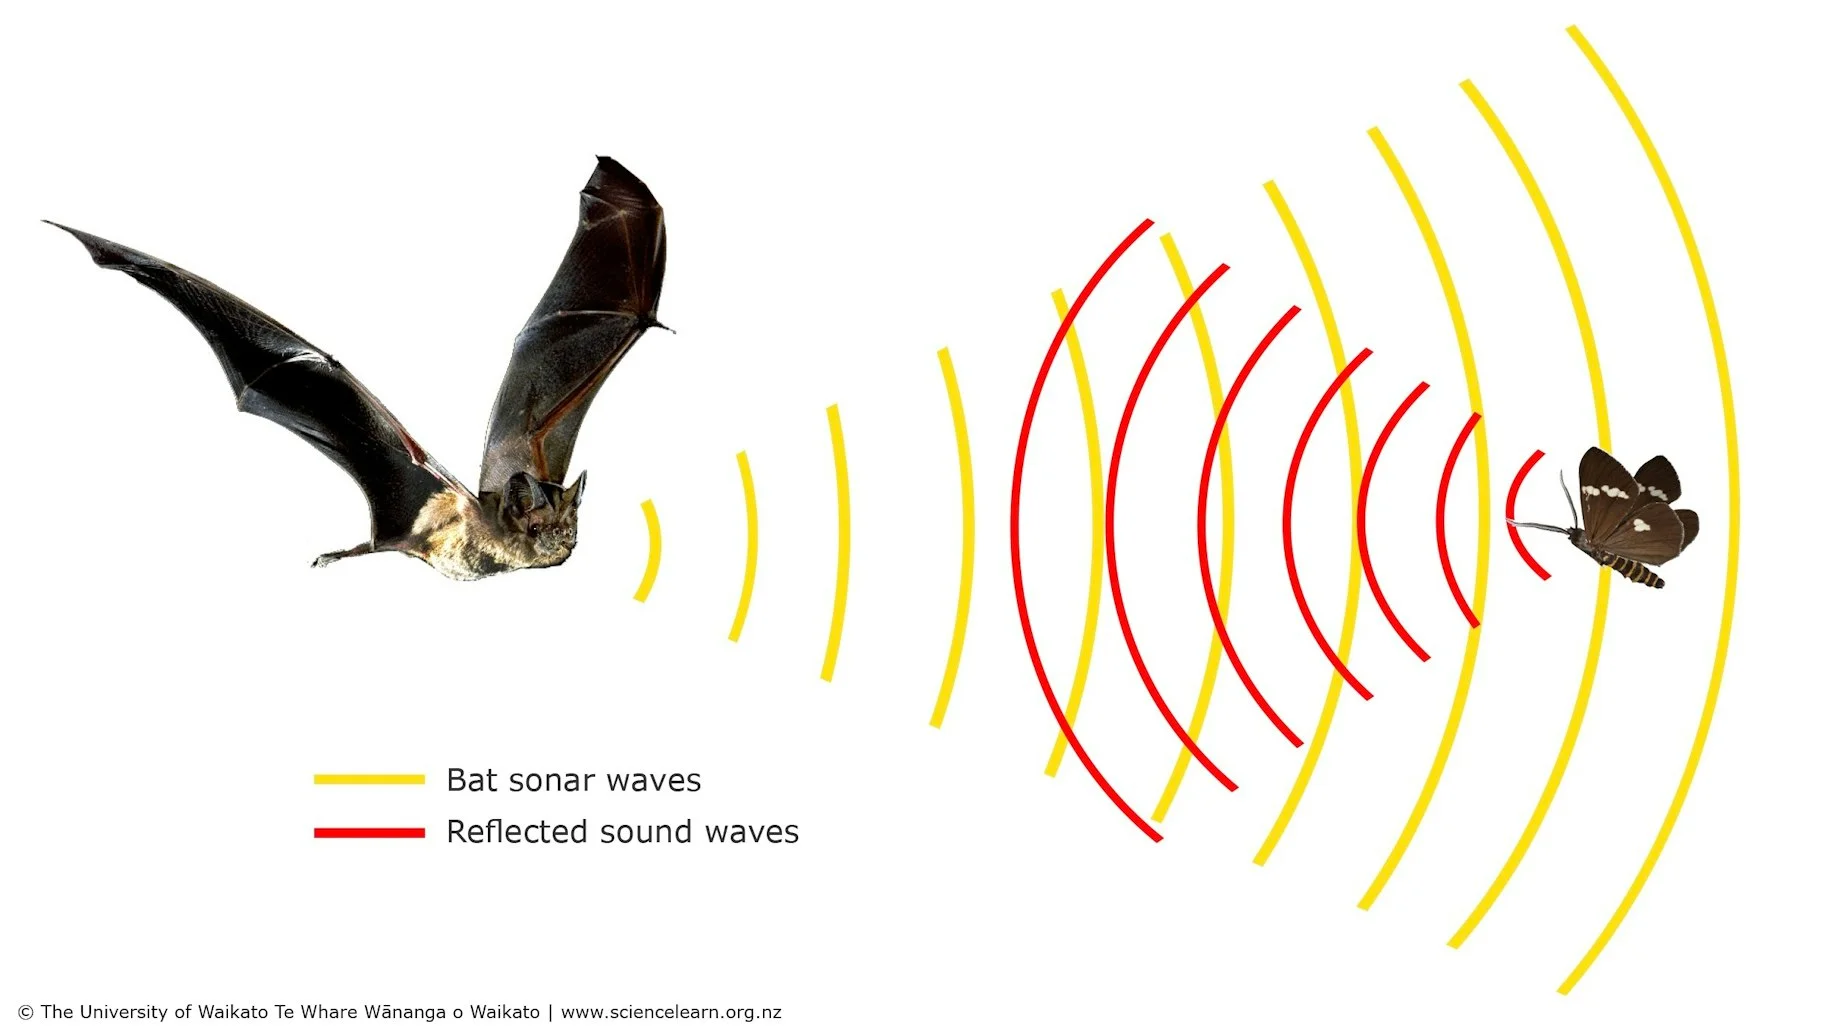
\includegraphics[width=0.72\linewidth]{2_Background/background_figures/Auditory_localisation/bat_echolocation.png}
    \caption{This diagram shows a bat, its ultrasound call, and the echo from an object, displaying the idea behind distance time of flight (ToF) cues \cite{BatHub}.}
    \label{fig:bat_echolocation}
\end{figure}


\subsection{Distance Cues}

In passive listening, estimating the absolute distance of a source using sound is highly error-prone because the initial source intensity is unknown. The brain must approximate range using
secondary acoustic markers, such as acoustic attenuation, atmospheric absorption, and reverberation. In short, this is the effect of how a sound changes through an environment, becoming quieter (attenuated), muffled (absorbed by the air), and elongated (reverb). An active echolocation system bypasses these cues in favour of a more informative one. By emitting
a self-generated pulse, the bat can measure the time it takes for the echo to return, known as time-of-flight (ToF). This can provide an explicit mapping to distance:

\begin{equation}
    r= \frac{c \cdot \text{ToF}}{2}
    \label{eq:tof_distance}
\end{equation}

where $r$ is the distance (or range) to the object, and $c$ is the speed of sound ($343 \text{m}\text{s}^{-1}$). This is the single most important cue for estimating distance, and measuring this accurately is more complicated than it first seems, particularly when using biological models. For example, how does biology create a simple timer? We will discuss this in section \ref{sec:biology}.

It should be noted that whilst other cues may indicate distance, such as the fact that the intensity of a sound attenuates with the square of the distance, these are often unreliable cues, and are usually controlled for rather than extracted as features. This is often the case for the other pathways as well.



\subsection{Azimuth Cues}
Localisation within the horizontal plane relies predominantly on binaural cues, which compare the differences between the acoustic signals arriving at the left and right ears. This is mainly dependent on interaural time difference (ITD), which is the time difference between the two ears, and interaural level difference (ILD), which is the level (volume) difference between the two ears. These ideas are shown in figure \ref{fig:azimuth_cues}. It should be noted that there are other cues to be considered, such as interaural phase difference, but we will discuss the primary cues that are implemented in the model developed.



\begin{figure}[H]
    \centering
    
    % Panel A
    \begin{subfigure}[t]{0.5\textwidth}
        \textbf{\large A}\\[0.5ex]  % Forces the bold 'A' to the top left
        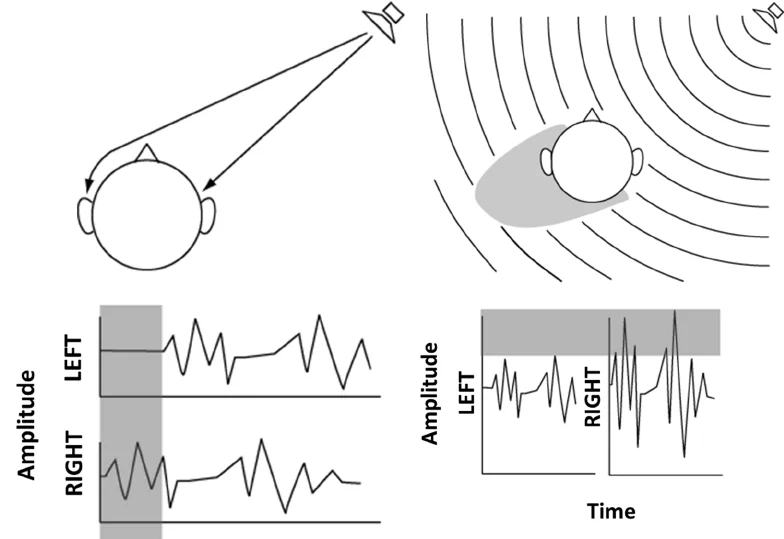
\includegraphics[height=5cm]{2_Background/background_figures/Auditory_localisation/itd_ild.png}
        \label{fig:itd_ild}
        \caption{}
    \end{subfigure}
    \hspace{0.1cm}
    % Panel B
    \begin{subfigure}[t]{0.3\textwidth}
        \textbf{\large B}\\[0.5ex]  % Forces the bold 'B' to the top left
        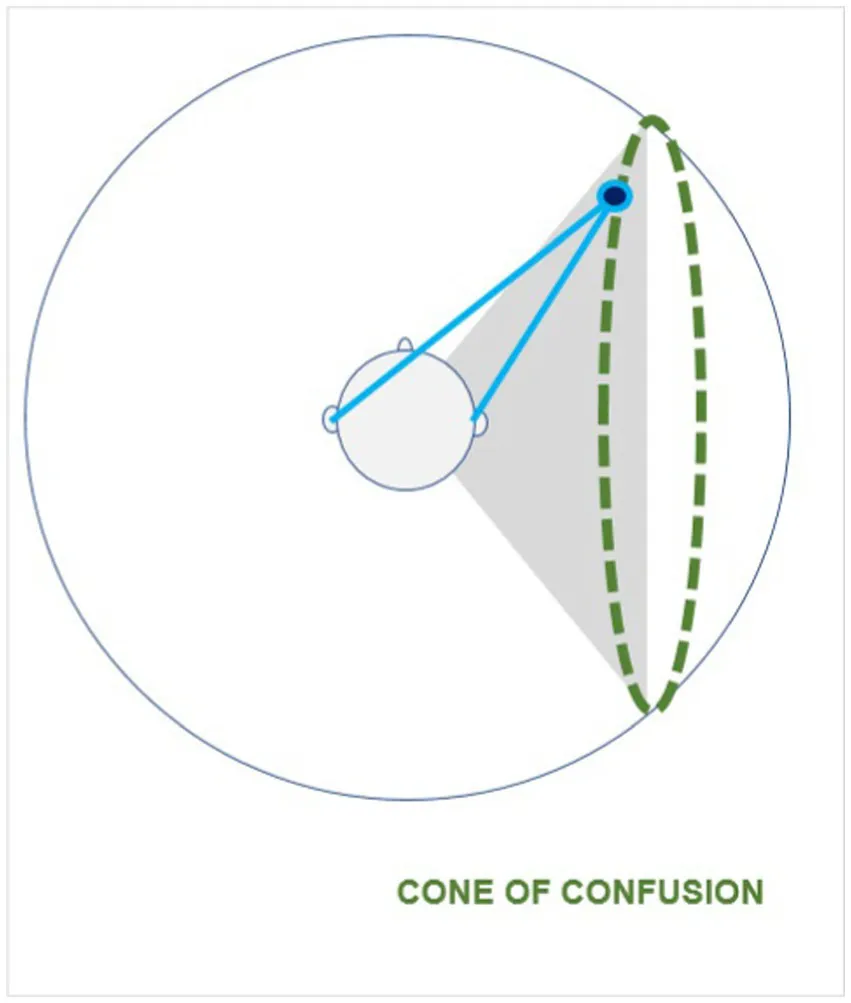
\includegraphics[height=5cm]{2_Background/background_figures/Auditory_localisation/cone.png}
        \caption{}
        \label{fig:cone}
    \end{subfigure}

    \caption{A: Interaural Time Difference (ITD) and Interaural Level Difference (ILD) \cite{Sun2015DynamicListeners}. B: Cone of confusion of constant ITD \cite{Carlini2024AuditoryReview}.}
    \label{fig:azimuth_cues}
\end{figure}

 \subsubsection{Interaural Time Difference (ITD)} When a sound source is located to one side, the acoustic wavefront travels a longer path to reach the farther ear. This path length difference creates an arrival time delay, or ITD. This can give a geometrical approximation of the azimuth:
\begin{equation}
    \theta = \arcsin\left(\frac{c \cdot \text{ITD}}{d}\right)
    \label{eq:itd_azimuth}
\end{equation}
where $d$ is the interaural distance. It should be noted that this is a straight line path approximation and does not account for the increased path length due to diffraction around the curvature of the head. This curvature would change the model to Woodworth's Model for ITD on a spherical head \cite{ExperimentalArchive}:
\begin{equation}
    \text{ITD} = \frac{d}{2c}(\theta + \sin\theta)
\end{equation}
Woodworth's Model cannot be inverted algebraically and requires numerical methods to calculate the azimuth from ITD. This is an example of how modelling complexities can be increased, but there are trade-offs to be considered. These trade-offs of simplifications will be discussed further in Chapter \ref{ch:modelling}.

One major limitation of pure ITD is that there is a cone of space where all ITDs are constant, as shown in figure \ref{fig:azimuth_cues}. This is often solved by combining the information from other cues, however, for pure tones of single frequencies, the side from which a sound originates can often be indistinguishable \cite{Rayleigh1907Direction}.

\subsubsection{Interaural Level Difference (ILD)} 
When the acoustic wavelength is shorter than the diameter of the head ($\lambda < d$), the sound wave cannot easily diffract around the structure. In this case, the head acts as an acoustic barrier, casting an ``acoustic shadow'' over the contralateral (far side) ear. This attenuates the sound amplitude at the far ear, creating an intensity difference. The difference in volume can ve used to estimate the angle of the sound source. Because it relies on acoustic shadowing, ILD is highly effective for high-frequency sounds. 

\subsubsection{Duplex Theory}
    
ITD is highly effective for low-frequency signals where the acoustic wavelength ($\lambda$) is significantly larger than the dimensions of the head ($\lambda > d$), as low frequencies can diffract much more easily. ILD is much more effective at high frequencies due to the acoustic shadow that forms. This idea is illustrated by Figure \ref{fig:duplex_theory}. For this reason, humans and mammals have evolved the ability to use both ITD and ILD cues for azimuth estimation of low and high frequencies, respectively. This transition between relying on low-frequency ITD and high-frequency ILD is known as the Duplex Theory of sound localisation \cite{Rayleigh1907Direction}. 

\begin{figure}[H]
    \centering
    
    % Panel A
    \begin{subfigure}[t]{0.45\textwidth}
        \textbf{\large A}\\[0.5ex]  % Forces the bold 'A' to the top left
        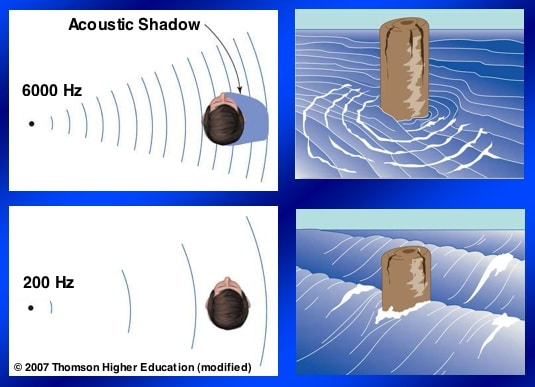
\includegraphics[height=7cm]{2_Background/background_figures/Auditory_localisation/waves.png}
        \label{fig:waves}
        \caption{}
    \end{subfigure}
    \hspace{3cm}
    % Panel B
    \begin{subfigure}[t]{0.2\textwidth}
        \textbf{\large B}\\[0.5ex]  % Forces the bold 'B' to the top left
        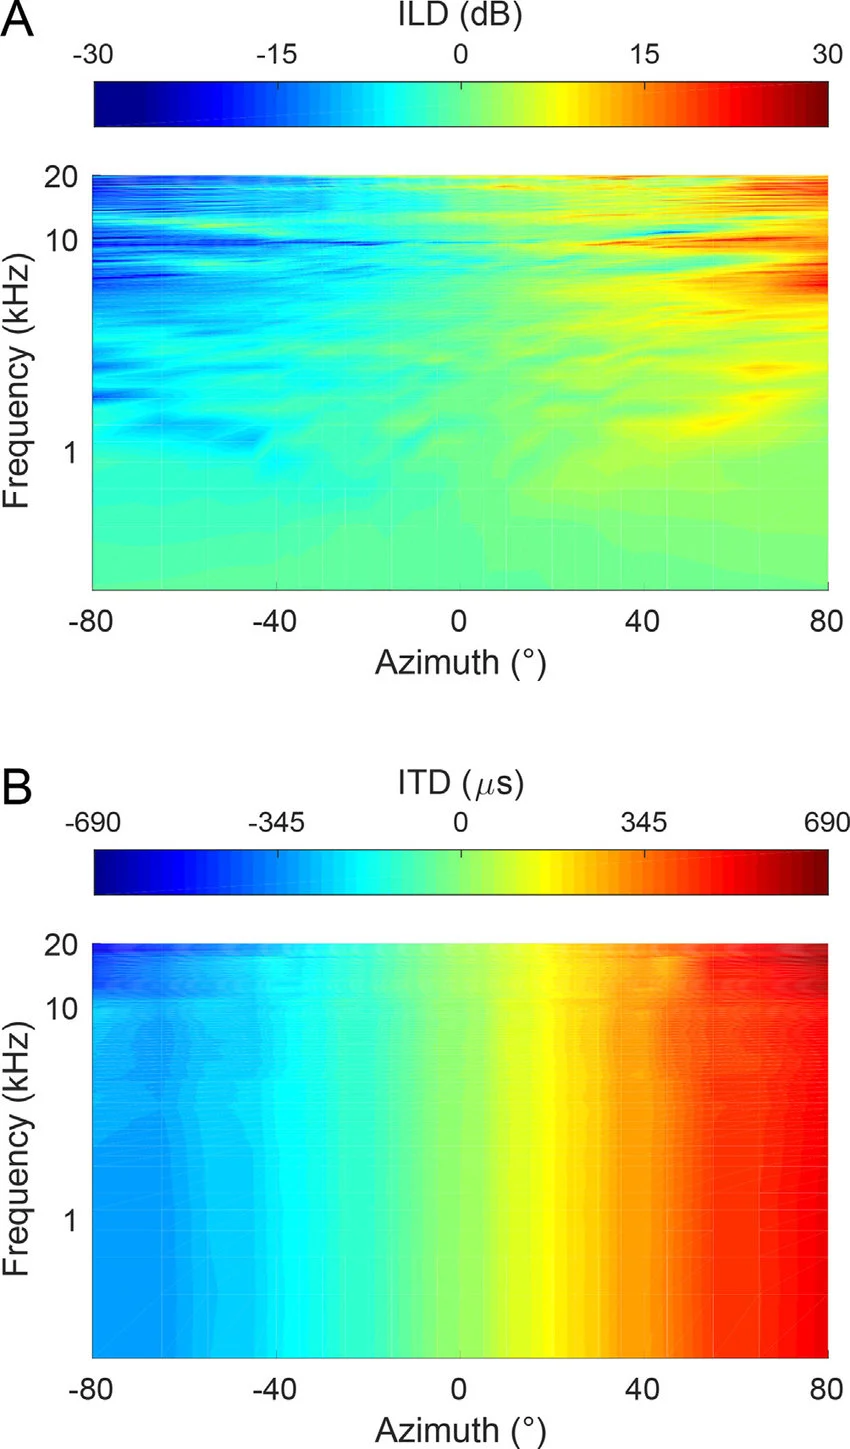
\includegraphics[height=7cm]{2_Background/background_figures/Auditory_localisation/duplex_contours.png}
        \caption{}
        \label{fig:duplex_contours}
    \end{subfigure}

    \caption{Head shadow effect is primarily active for high frequency sounds that have short wavelengths and meet resistance and absorption when encountering the head. Low frequency sounds have long wavelengths, are able to diffract around the head, and therefore have less significant interaural intensity differences. A: \cite{HowLocalization}. B: \cite{Kumpik2019AHearing}. YOU DONT MODEL THIS, REMOVE?}
    \label{fig:duplex_theory}
\end{figure}


\subsection{Elevation Cues}

Due to the symmetric skull of most species, binaural cues vary mostly in the horizontal plane. This means vertical localisation often relies purely on monoaural spectral cues \cite{Kumpik2019AHearing}. The asymmetrical, complex cartilage of the outer ear (the pinna) acts as an acoustic directional filter. As sound waves strike the ridges of the pinna, they reflect and interfere destructively or constructively depending on their angle of incidence. This introduces direction-specific spectral peaks and notches into the frequency profile, as shown in Figure \ref{fig:elevation_cues}. This type of interference is often called comb filtering. This spectral filtering also happens in the horizontal plane, solving the problem of the cone of confusion through spectral differences. This also explains why pure tones are much harder to locate than broadband sounds, such as speech.


\begin{figure}[H]
    \centering
    
    % Panel A
    \begin{subfigure}[t]{0.45\textwidth}
        \textbf{\large A}\\[0.5ex]  % Forces the bold 'A' to the top left
        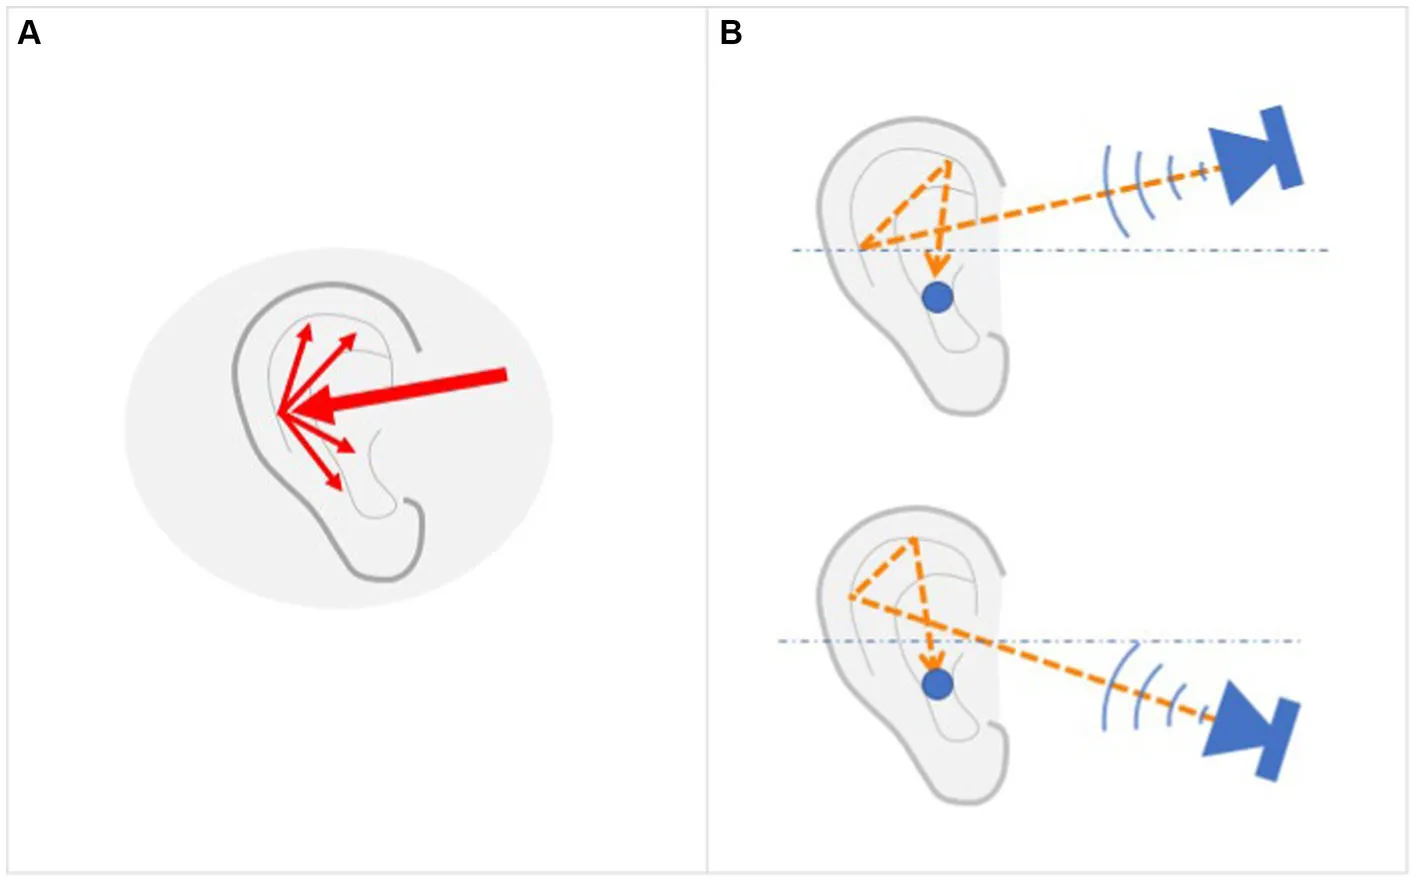
\includegraphics[height=4cm]{2_Background/background_figures/Auditory_localisation/pinna_1.png}
        \label{fig:pinna}
        \caption{}
    \end{subfigure}
    \hspace{0.1cm}
    % Panel B
    \begin{subfigure}[t]{0.45\textwidth}
        \textbf{\large B}\\[0.5ex]  % Forces the bold 'B' to the top left
        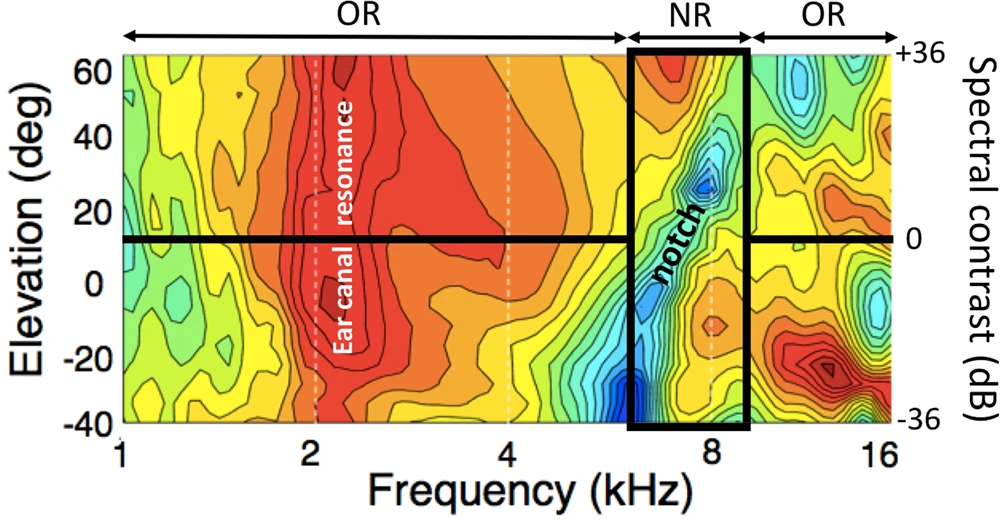
\includegraphics[height=4cm]{2_Background/background_figures/Auditory_localisation/pinna_map.png}
        \caption{}
        \label{fig:pinna_map}
    \end{subfigure}

    \caption{A: Mechanics of Head Related Transfer Function (HRTF) due to the pinna \cite{Carlini2024AuditoryReview}. B: Color-coded HRTFs for elevation. High gain in red and low gain in blue. OR: outer region. NR: notch region \cite{Zonooz2019SpectralElevation}.}
    \label{fig:elevation_cues}
\end{figure}


This combined effect of the head on monoaural and binaural cues is known as the Head Related Transfer Function (HRTF), and describes the general transfer function due to the head being physically in between the two ears, with complex pinna acting as directional filters. The HRTF is complex and unique for everyone, making it difficult to model and simplify. 


\subsection{Auditory Cues and Signals for Bats}

Bats use many of the same auditory cues as other mammals, but have evolved to take advantage of the key aspects of the cues. Echolocatory bats (which will be the only bats we refer to) use high-frequency ultrasound calls in order to minimise the diffraction around small objects, such as insects, and to create a highly detailed sonar map. They use a frequency modulated (FM) sweep to make full use of the spectral cues, using them for object position, structure, and shape. Some bats also use a constant frequency component in their calls to harness the Doppler effect to track the velocity of insects. Examples of these are shown in Figure \ref{fig:bat_call}. The balance between the CF and FM components of a bat's call is a close reflection of the specific bat's environment and hunting style, meaning every bat has a unique call \cite{Beetz2022NeuralBats}. Figure \ref{fig:bat_call} also shows the increase in pulse rate as the bat approaches the prey. This demonstrates how bats take ``snapshots'' of their prey's position in decreasing intervals.

\begin{figure}[H]
    \centering
    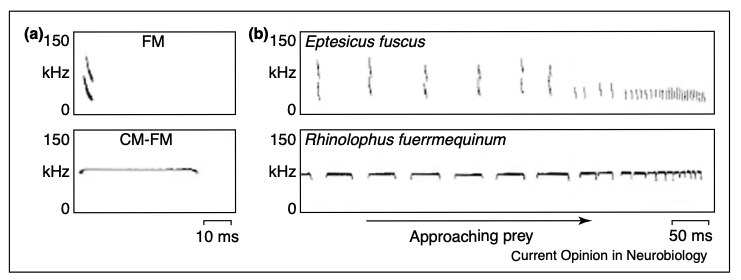
\includegraphics[width=0.9\linewidth]{2_Background/background_figures/Auditory_localisation/bat_call.png}
    \caption{Echolocation signal structures. (a) Spectrographic examples of frequency modulated (FM) and constant frequency (CF) signal components used by echolocating bats. (b) Spectrographic sequence of signals produced by an FM-bat, Eptesicus fuscus and a CF-FM bat, Rhinolophus ferrumequinum, while pursuing insect prey. Typical of insectivorous echolocating bats, signal repetition rate increases and the duration decreases as the animal approaches its prey \cite{MossANeurobiologyBats}.}
    \label{fig:bat_call}
\end{figure}

Due to the high frequency of a bat's call, some species of bats utilise ILD cues much more than ITD for azimuth estimation, however this is not applicable to all bats, as their small heads make diffraction still possible. Bats also utilise the Lombard effect, which is simply using louder calls in noisy environments \cite{Pedersen2024SuperfastBats}.

The bat's brain is responsible for using these auditory cues and inferring position from them. It does this using complex neural circuitry, as discussed in Section \ref{sec:biology}.







\section{Biological Foundations of Echolocation} \label{sec:biology}

In this section, we will look at the biological pathways in which the bat's brain computes echolocatory signals. The objective of this section is not to provide an exhaustive anatomical survey of the chiropteran brain, but rather to isolate the core computational principles, structural constraints, and functional logic found in biological auditory systems. By abstracting these biological mechanisms into discrete signal-processing blocks, we establish a direct architectural framework for the neuromorphic model developed in Section \ref{ch:modelling}. 


\subsection{Biological Neurons: The Basics of Biological Computation}

In order to discuss the auditory pathways of a bat's brain, we must understand the building blocks of biological computational systems. The key systems are:
\begin{enumerate}
    \item \textbf{Action Potentials:} Action potentials are the signals that get transmitted around biological circuits. These are asynchronous, event-driven, binary signals that are often referred to as ``spikes'' to reflect their sharp increase and decrease of voltage.
    \item \textbf{Neurons:} Neurons are like the wires in biological circuits that carry the action potential signals.
    \item \textbf{Synapses:} Synapses are like the switches or logic gates in biological networks. They transfer the signal from one neuron to another, with varying strength.
    \item \textbf{Inhibition:} Action potentials cannot be negative, and so inhibitory signals are transmitted using chemicals that reduce the excitation of surrounding neurons. These will often be discussed in a similar manner to the excitatory action potential signals, however, they are fundamentally a different mechanism.
\end{enumerate}
We will often discuss biological circuits with reference to electrical circuits, which is often helpful for understanding, however, it is important to understand that no continuous signals are sent, and all signals are made up of spiking action potentials.

It is also important to note that a lot of the functions of different brain areas are vast simplifications of the intricate and complex real biological functions. Part of the work of this project has been to decipher and simplify the true functioning of these brain areas into understandable, implementable uses.


\subsection{Neurobiology Overview}
To transition from a raw, physical acoustic echo to a localised spatial coordinate, the microchiropteran brain processes signals through an intricate, parallelised network of neurons and brain areas. This architecture functions as an assembly line of specialised computing units, where raw sensory streams are progressively processed.

Figure~\ref{fig:overall_pathway} illustrates the structural topology of the ascending and descending auditory systems of the Microchiroptera neurobiology. This specific wiring diagram serves as the structural blueprint for the synthetic SNN model developed in this work. Rather than building a single monolithic network, the modeling approach directly mirrors this biological division of labor: a uniform front-end peripheral network handles sensory spike encoding, which then diverges simultaneously into three parallel, feature-specific midbrain processing pipelines for distance, azimuth, and elevation extraction. 

\begin{figure}[h]
    \centering
    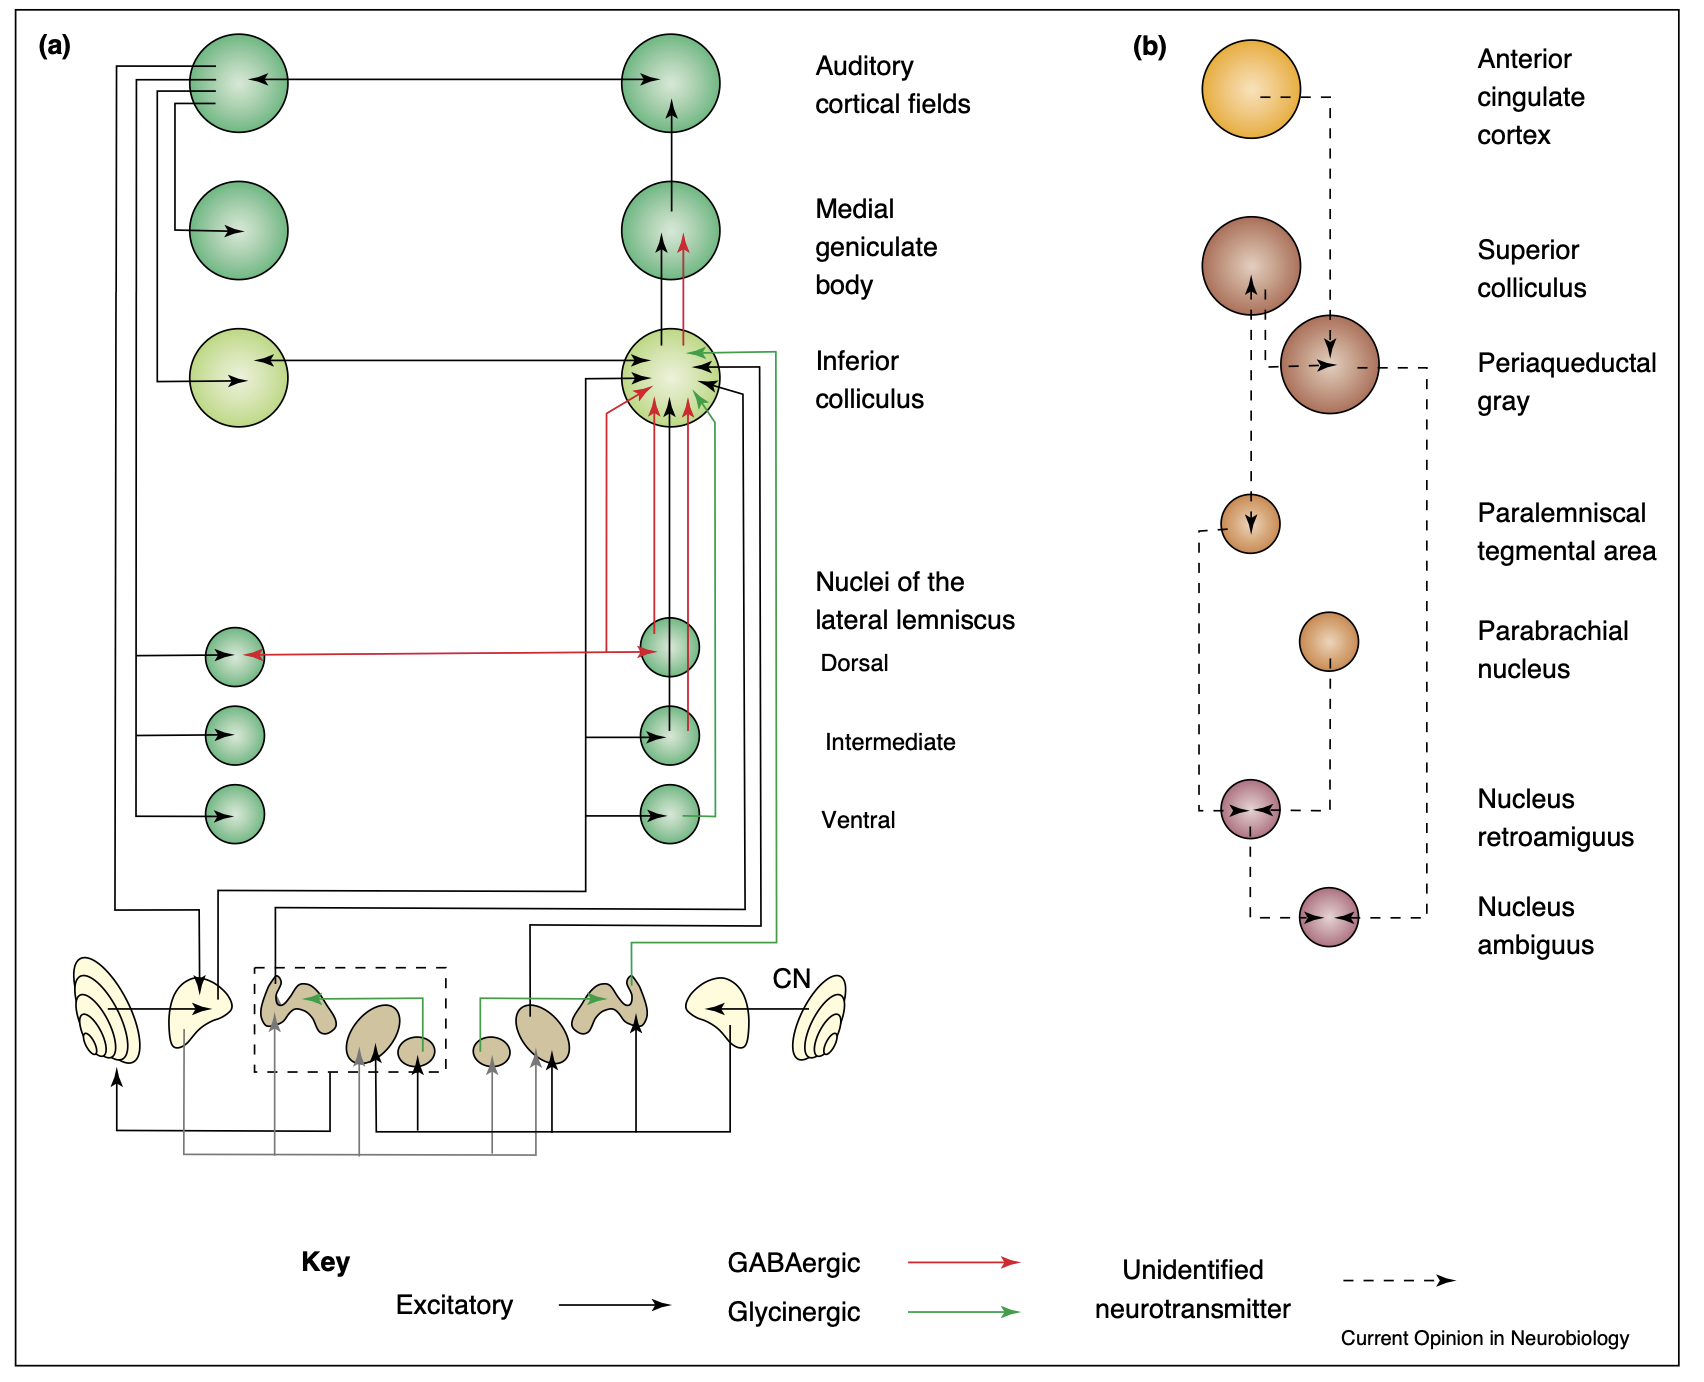
\includegraphics[width=\textwidth]{2_Background/background_figures/biology/overall_brain.png}
    \caption{Major connections of the (a) ascending auditory system, and descending auditory corticofugal projections. The dashed box demarcates nuclei of the superior olivary complex (SOC) that includes the lateral superior olive, the medial; superior olive and the medial nucleus of the trapezoid body. (b) Selected projections of vocal production circuitry from cited works. Excitatory projections are shown with black lines, inhibitory GABAergic projections are shown with red lines, inhibitory glycinergic projections are shown with green lines, and connections with as yet unidentified neurotransmitters are shown with dashed black lines. Abbreviations: CN, cochlear nucleus. \cite{MossANeurobiologyBats}}
    \label{fig:overall_pathway}
\end{figure}

While current state-of-the-art biological auditory models often prioritise hyper-realistic, biophysical simulations using partial differential equations to track cochlear fluid mechanics, this report focuses on an alternate engineering objective: extracting the underlying neuromorphic algorithms required to implement an end-to-end spatial localisation.

\subsection{Vocalisation Pathway}

The diagram on the right of Figure \ref{fig:overall_pathway} shows the vocalisation pathway and the corticofugal (meaning the direction is outwards from the brain to the body) projections. The Anterior Cingulate Cortex (ACC) is the effective trigger for a voluntary call, which sends a signal to activate the Periaqueductal Gray (PAG). This acts as a gating mechanism for the Nucleus Ambiguus (NA), which connects to the laryngeal muscles via the laryngeal nerve, essentially telling it when to make a bat call. 

The Superior Colliculus (SC) is the most important brain area in the vocalisation pathway for this report. It handles the 3D sensorimotor map, and coordinates when and how long a sonar pulse needs to be emitted to optimise localisation. The SC receives signals from the effective outputs of the position coordinate pathways, essentially acting as the centralised readout centre of the pathways. This readout for the bat is the bat's perception of the world, and is used to coordinate the muscles and echolocatory systems.

The SC projects the sensory measurement information to the Paralemniscal Tegmental Area (PLA). The PLA helps formulate this into motor commands and works to shape the precise acoustic properties of the pulse. 

The Parabrachial Nucleus (PBN) is responsible for the autonomic respiratory control. The PBN and PLA converge on the Nucleus Retroambiguus (NRA) in the medulla. This acts as the coordinator for the muscles in order to exhale air and tighten the vocal cords in the desired manner. This projects to the NA, contracting the muscles in a desired way to control the tension of the muscles, altering the pitch and envelope of the bat's call, essentially telling it how to design the bat call.

This is a complicated process involving sensory and motor feedback control, and is included to highlight the vast simplifications that will be made in the model. It also shows how a complex neural system can be designed for a singular task, a coordinated task.

Aside from the SC, the most important part of this system is something called the Corollary Discharge (CD). This is the process that sends a copy of the spiking signal that is expected to be received (called an efference copy), in order for the processing pathways to compare this copy to the received and decoded echo signal. This is believed to originate in the SC, which sends/projects it to the PAG and PLA, which in turn send it further. This CD efference copy ends up throughout the auditory pathways, blocking the reception of the outgoing call, and preparing the brain for the incoming echo.


\subsection{The Auditory Frontend: Peripheral and Hindbrain Processing}

Once the bat call has been sent, and the CD distributed, the processing pathways (shown on the right of Figure \ref{fig:overall_pathway}) take the raw waveform, and from this, infer the position of the object that reflected the echo.

\subsubsection{Cochlea}

First, the raw waveform must be encoded into spikes - the language of our biological circuits. The cochlea is the biomechanical transducer of the auditory system, and the system that does this task. Mechanically, it operates as a hydrodynamic frequency analyser. Incoming acoustic pressure waves first pass through the outer ear, which performs the spectral filtering discussed earlier. The middle ear then performs impedance matching, often by contracting the middle ear muscles (MEM) (such as the stapedius) in what is known as the MEM reflex \cite{Winter2023PartCambridge}. Bats have the unique ability, unlike humans, to voluntarily contract these muscles to protect the ear from the loud sound of their call, and then progressively relax it, which helps match the impedance to the volume of the expected echo, which will decrease with time.


\begin{figure}[H]
    \centering
    
    % Panel A
    \begin{subfigure}[t]{0.45\textwidth}
        \textbf{\large A}\\[0.5ex]  % Forces the bold 'A' to the top left
        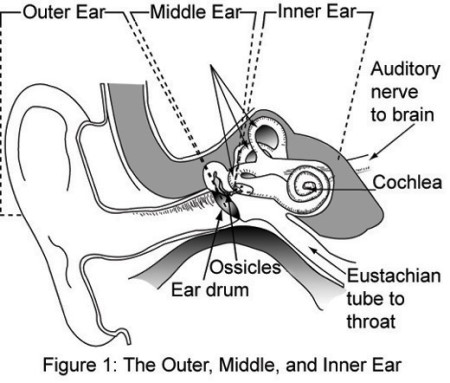
\includegraphics[height=4cm]{2_Background/background_figures/biology/cochlea.png}
        \label{}
        \caption{}
    \end{subfigure}
    \hspace{0.1cm}
    % Panel B
    \begin{subfigure}[t]{0.45\textwidth}
        \textbf{\large B}\\[0.5ex]  % Forces the bold 'B' to the top left
        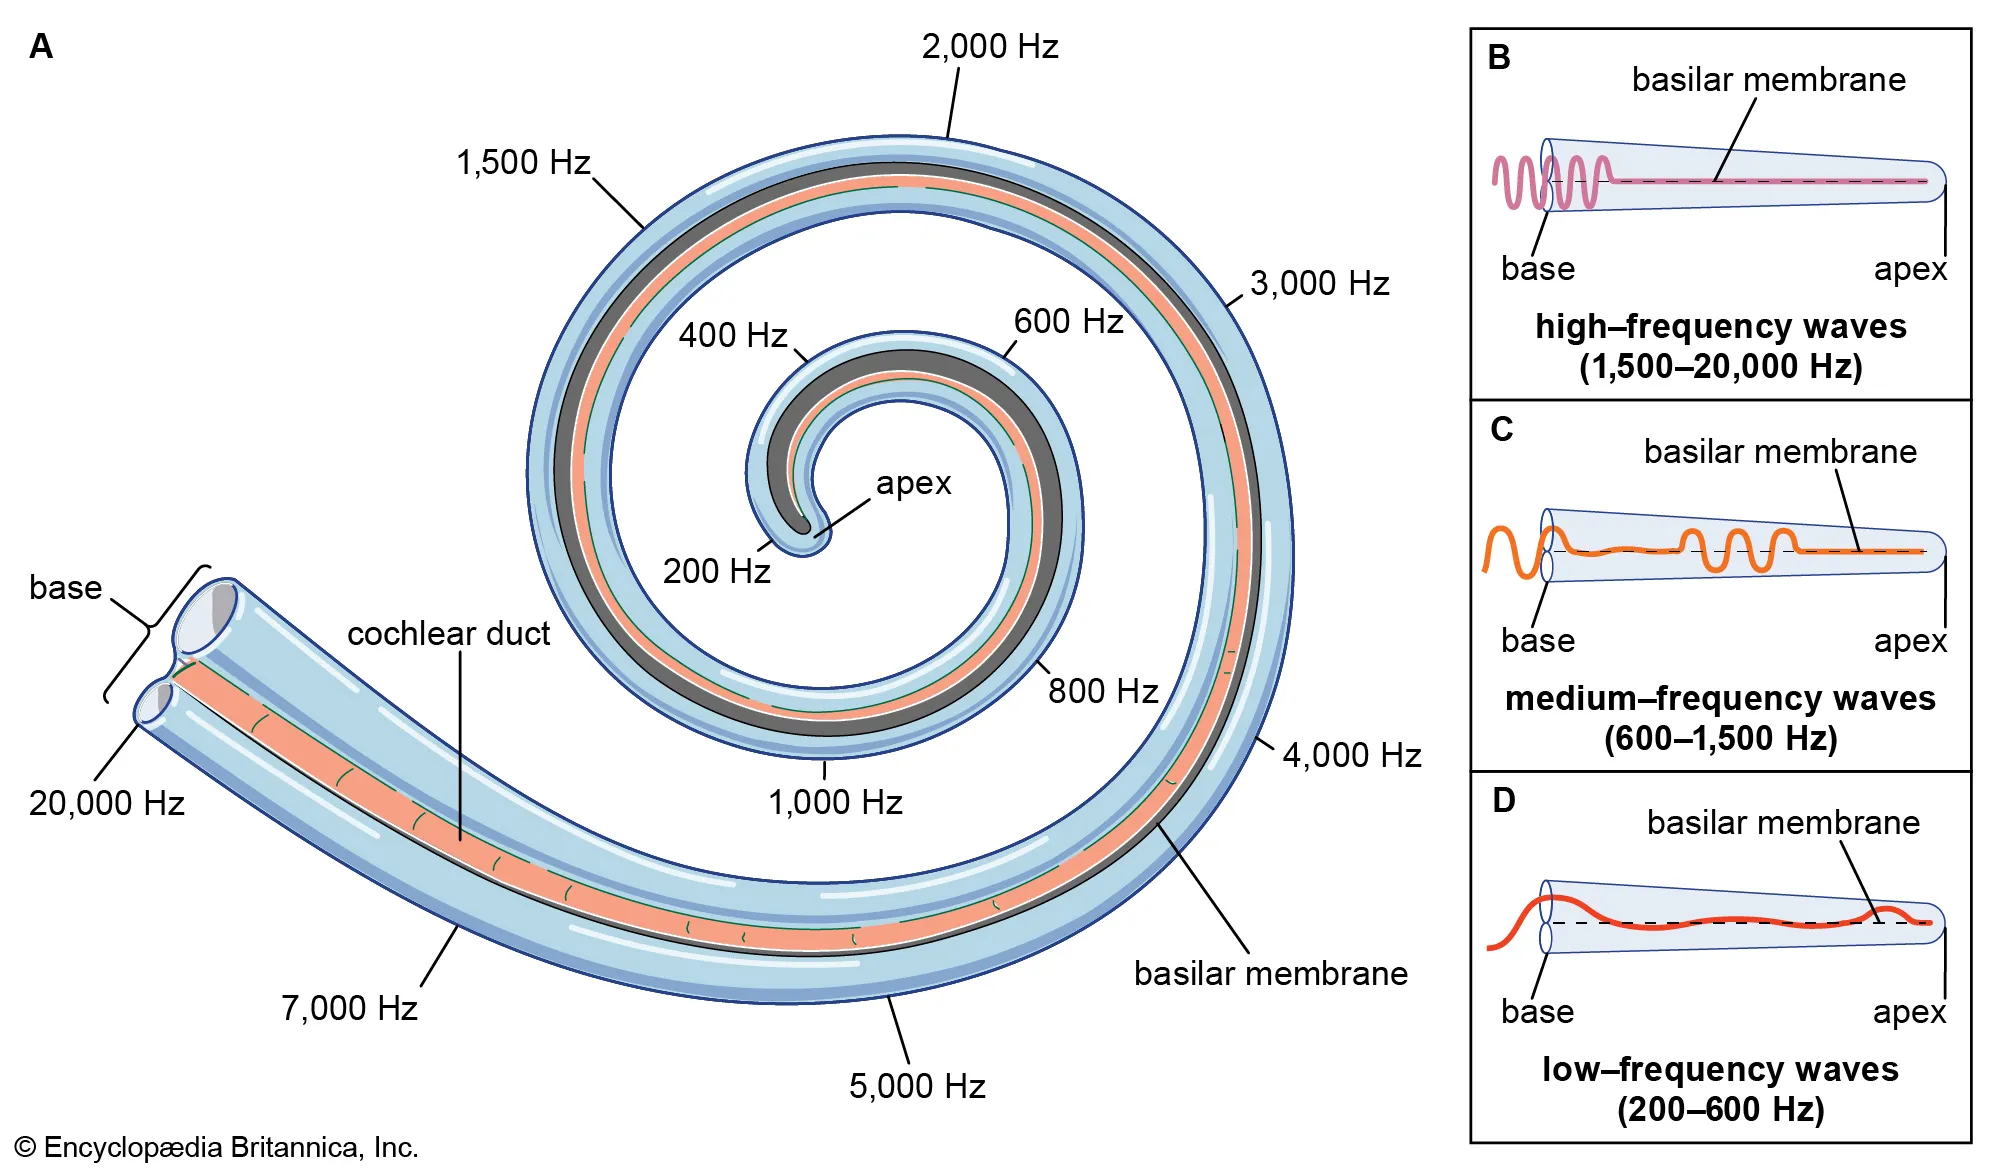
\includegraphics[height=4cm]{2_Background/background_figures/biology/spiral.png}
        \caption{}
        \label{}
    \end{subfigure}

    \caption{A: The Outer, Middle, and Inner Ear  \cite{CochleaStudy.com}. B: Cochlea Spiral frequency place coding, and basilar membrane \cite{HumanBritannica}. Whilst both these diagrams are for the human ear, the understanding is the same and applicable to the bat}
    \label{fig:cochlea}
\end{figure}

The sound waves then travel into the inner ear and the cochlea. Here they travel along the basilar membrane, which varies continuously in width and stiffness from its base to its apex. This variation generates a spatial gradient of resonance: high frequencies create peak displacements near the rigid base, while low frequencies propagate to the flexible apex. This is known as spatial frequency dispersion. The outer hair cells, which sit on the outside of the basilar membrane, help amplify this resonance. The fluid inside the basilar membrane then moves the inner hair cells, which, when moved, trigger spiking action potentials that travel along the auditory nerve to the Cochlear Nuclei (CN).

\subsubsection{Cochlear Nuclei}
The auditory nerve terminates directly within the CN, the primary hindbrain processing station. The CN acts as the master router of the auditory system. It takes the single tonotopic spike stream from the ear and duplicates it across three major specialised sub-nuclei, each optimising the signal for a completely different downstream computational task.

\
\begin{figure}[H]
    \centering
    
    % Panel A
    \begin{subfigure}[t]{0.45\textwidth}
        \textbf{\large A}\\[0.5ex]  % Forces the bold 'A' to the top left
        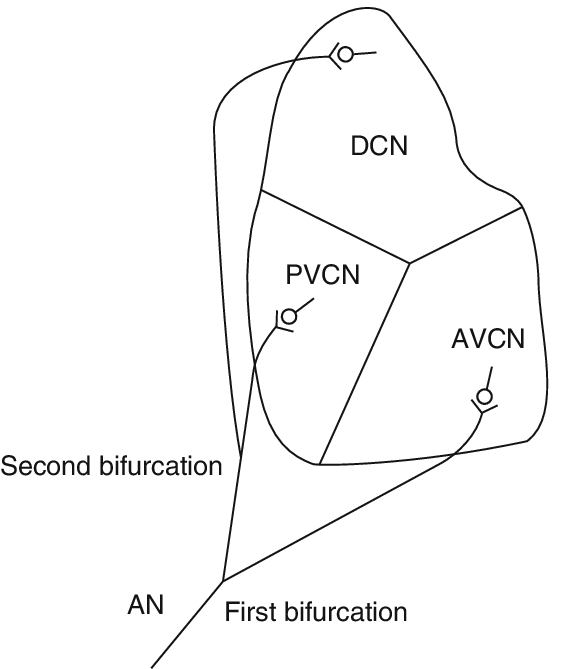
\includegraphics[height=4cm]{2_Background/background_figures/biology/CN.png}
        \label{}
        \caption{}
    \end{subfigure}
    \hspace{0.1cm}
    % Panel B
    \begin{subfigure}[t]{0.45\textwidth}
        \textbf{\large B}\\[0.5ex]  % Forces the bold 'B' to the top left
        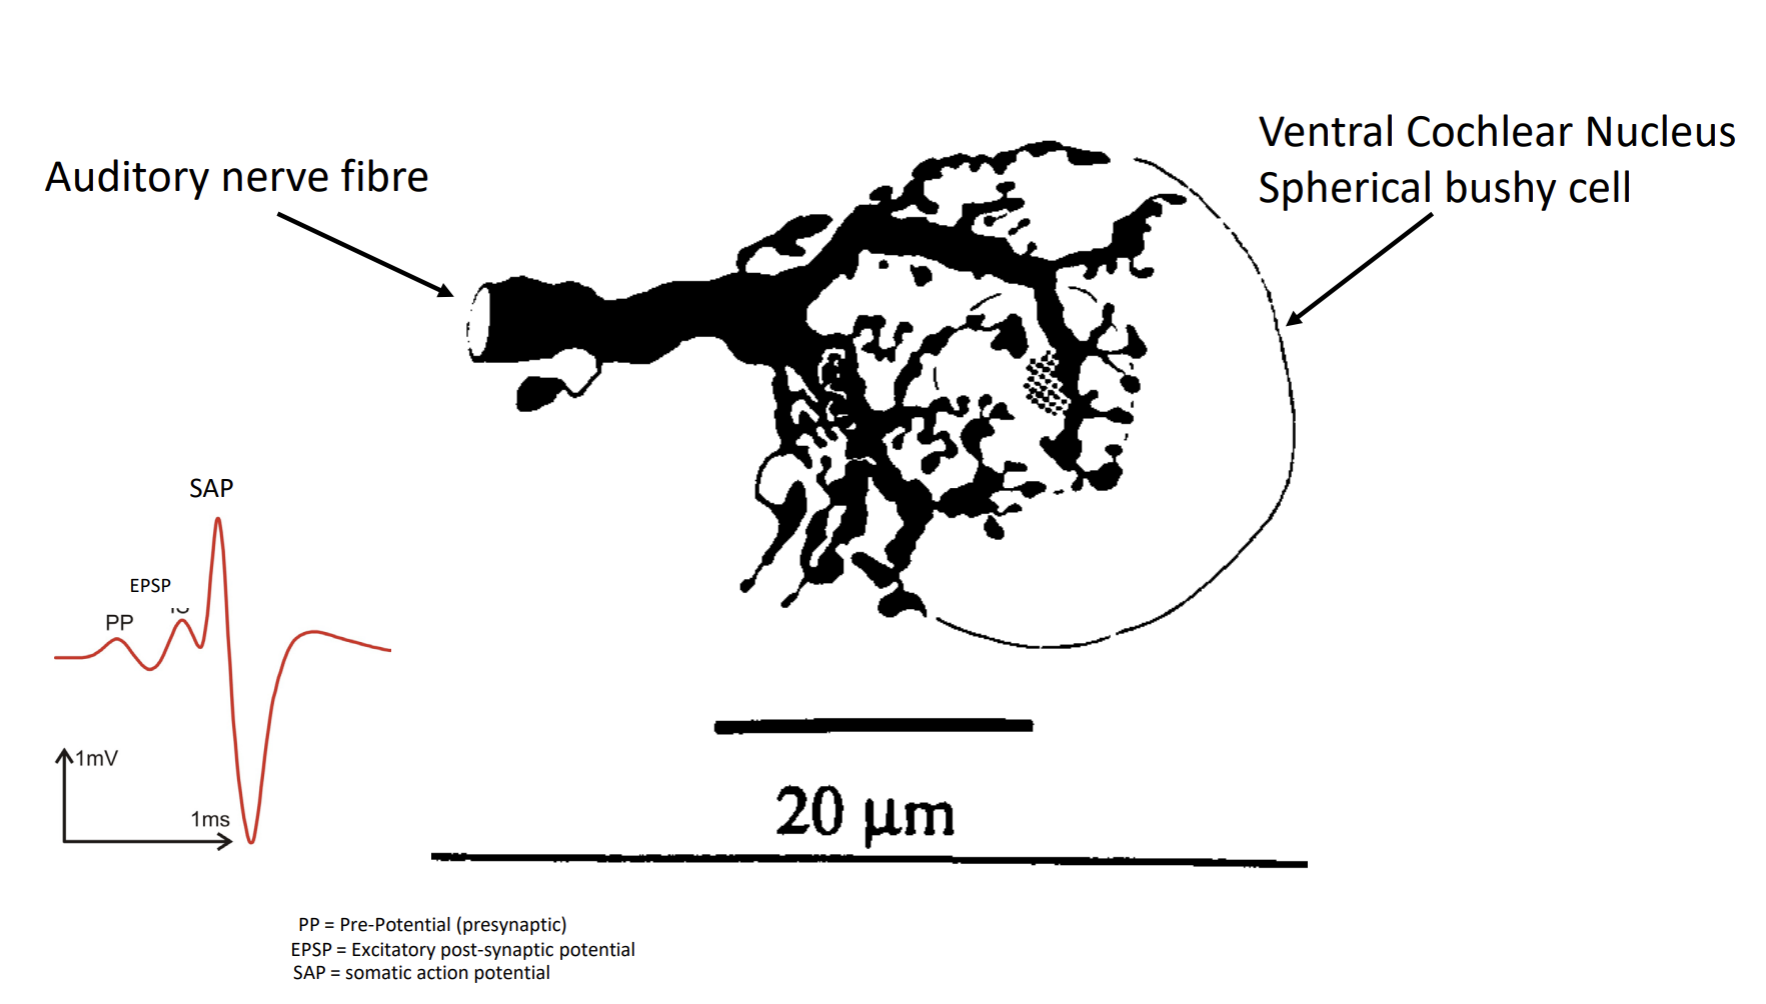
\includegraphics[height=4cm]{2_Background/background_figures/biology/endbulb.png}
        \caption{}
        \label{}
    \end{subfigure}

    \caption{A: Schematic drawing of the cochlear nucleus to show the auditory nerve's connections with the three main divisions and the cochlear nucleus. DCN dorsal cochlear nucleus, PVCN posterior ventral cochlear nucleus, AVCN anterior ventral cochlear nucleus.  \cite{Mller2011AnatomySystem}. B: The endbulb of Held \cite{Winter2023PartCambridge}.}
    \label{fig:CN}
\end{figure}


\paragraph{Ventral Cochlear Nucleus (VCN):} 
The VCN handles the preservation of timing and intensity details. It is structurally bifurcated into two primary functional components:
\begin{itemize}
    \item \textbf{Anteroventral Cochlear Nucleus (AVCN):} The AVCN is dominated by spherical and globular bushy cells. These neurons feature exceptionally massive, secure synaptic connections known as the Endbulbs of Held, which are the biggest fastest synapses in the brain (see Figure \ref{fig:CN}) \cite{Winter2023PartCambridge}. These specialised synapses exhibit minimal jitter (temporal fluctuations) and ultra-fast recovery times, allowing the cells to replicate the firing patterns of the auditory nerve with sub-millisecond temporal fidelity. The AVCN exists to preserve precise temporal phase and timing information, acting as the primary input engine for the binaural azimuth pathway.
    \item \textbf{Posteroventral Cochlear Nucleus (PVCN):} The PVCN is characterized by octopus and stellate cells. Octopus cells act as global onset detectors. They possess wide dendritic trees that pool spikes across a broad range of frequency channels. When a rapid wideband signal, such as an FM echolocation sweep, strikes the periphery, these cells integrate the incoming wavefront and discharge a single, hyper-precise ``onset spike''. This provides a clean, unambiguous temporal anchor marking the exact arrival time of the echo, which is critical for distance calculation. Stellate cells encode volume by having multiple neurons, each with varying thresholds for spiking. This means higher volume signals cause more neurons to spike.
\end{itemize}

\paragraph{Dorsal Cochlear Nucleus (DCN):}
In stark contrast to the timing-focused VCN, the DCN features a highly stratified, complex internal circuitry that operates as an adaptive spectral analyser. The DCN processes monaural spectral cues by combining direct acoustic inputs from the cochlea with inhibitory feedback from internal interneurons. 

Its primary computational objective is to extract the direction-specific spectral notches and peaks imposed on the echo by the bat's pinna (the HRTF). By identifying how these notches shift in frequency space, the DCN extracts a raw spectral fingerprint that maps directly to the vertical elevation of the target. This pre-filtered spectral landscape is passed directly to the midbrain for elevation mapping.


\subsection{The Distance Pathway: Measuring Temporal Interval}
\label{sec:distance_pathway}
Target distance (range) estimation in active echolocation is fundamentally a problem of ToF estimation. The central nervous system must calculate the temporal interval between the broadcast of the vocalisation and the arrival of the returning echo, mapping this delay to a physical distance. This means they must retain signals in their brain for extended periods of time, as a biological timer. This is the fundamental idea behind the distance pathway.

The distance pathway starts by using the precise temporal encoding of spikes from the VCN. The latency of these is naturally volume-dependent, meaning louder signals cause spiking sooner. This is an issue for precise ToF timing. The signals from the VCN then travel to the Nuclei of the lateral lemniscus (NLL), as well as the INferior Colliculus (IC). The NLL has three major components to it:
\begin{itemize}
    \item Ventral Nucleus of the lateral lemniscus (VNLL): This has a monoaural effect of correcting the volume-dependent latency from the VCN by using inhibitory signals. It is vital for temporal precision, and when combined in the IC, the VCN and the VNLL effectively have constant latency.
    \item Intermediate Nucleus of the lateral lemniscus (INLL): This is also monoaural, and has excitatory and inhibitory behaviour. It aids in spectral feature extraction and spectral suppression.
    \item Dorsal Nucleus of the lateral lemniscus (DNLL): This is binaurally connected, and from receiving signals from the VCN, sends a long-lasting inhibitory signal to the IC, which suppresses reverberation and echoes that are received after the primary echo.
\end{itemize}
The NLL is also the primary inhibitory centre, which diffuses the inhibitory signal from the corollary discharge.

Within the IC, temporal intervals are converted into a spatial topographic representation via delay-tuned neurons (specifically categorised as FM-FM neurons). These cells are highly non-linear coincidence detectors: they remain completely silent when stimulated by the pulse or echo alone, but exhibit a massive, facilitated response when the two signals arrive at a specific, characteristic delay interval. If the physical time-of-flight of the echo perfectly matches the internal propagation delay of the pulse channel, the two electrical inputs arrive at the post-synaptic IC neuron simultaneously. This exceeds the firing threshold, releasing a localised spike. The coincidence detectors and FM-FM neurons in the IC are unorganised and do the raw timing arithmetic, and send sharpened versions of the resulting signals to the auditory cortex (AC).

The AC is the organiser of this messy arithmetic. They also contain FM-FM delay tuned neurons, however these ones are tonotopically organised. This means there is effectively a 2D map in the bat's brain which accounts for volume and distance of each signal. The output of the AC is sent to the SC, which initiates the feedback control loop to send the next pulse.

\subsubsection{The Simmons-Suga Hyperacuity Debate}
The workings of these delay-tuned neurons is a long-disputed controversy between two models initially developed by  James Simmons and Nobuo Suga:
\begin{itemize}
    \item {The Suga Model (Discrete Templates):} This is the anatomical argument. This hypothesises that distance is represented by an array of rigidly pre-wired, discrete neural delay lines. Neurons are mapped to specific millisecond intervals (e.g., 1~ms, 2~ms, 3~ms), meaning resolution is fundamentally bounded by the density and step-size of the physical templates. The argument for this model is that the neurons have been physically found and tested to behave like this.
    \item \textbf{The Simmons Model (Hyperacuity Phase-Correlation):} This is the performance argument. Despite the anatomy showing relatively large discrete jumps in timing, the behavioral tracking of bats displays a hyperacuity down to tens of nanoseconds, arguing that the auditory system performs an active, continuous cross-correlation or phase-coherent spectral analysis that goes far beyond discrete millisecond delay lines.
\end{itemize}
 This debate is still ongoing, and so modelling this phenomenon is more difficult. The current most popular theory for this population coding, where the activity of neurons across a population can be averaged out to give higher resolutions. The method in which this is done is still disputed.


\subsection{The Azimuth Pathway: Binaural Disparity Processing}
\label{sec:azimuth_pathway}
TO DO

\subsection{The Elevation Pathway: Monaural Spectral Mapping}
\label{sec:elevation_pathway}
TO DO









\section{Neuromorphic Computing}
TO DO

\subsection{Computing with Spikes}

\subsubsection{Spikes and Encoding}


\subsubsection{Neurons: Mathematical Implementations}


\subsubsection{Neuronal Structures: Computational Analogies}


\subsection{Continuous Attractor Neural Networks (CANN)}


\subsection{Spiking Neural Networks and Deep Learning}


\subsection{Neuromorphic Hardware Compatibility}


\section{Current Biomimetic Models of Echolocatory Bats}














